\chapter{Projects}

\section{STM32 IMU}
\subsection{PModNav}
The purpose is to get the \texttt{roll}, \texttt{pitch} and \texttt{yaw} from the PModNav to plot a 3D visualization of the IMU. The final purpose of it is to create log files from the orientation and attitude of the drone in real-time. By combining data from accelerometers, gyroscopes and magnetometers, an IMU can provide information about the object's position, orientation and angular velocity. This is crucial for tasks such as safety deployement or drone tracking.
The STM32-L4796ZG recovers the value of the sensors from the \texttt{PModNav} via \texttt{SPI Bus} and transmits them to the HMI via \texttt{UART} connection.
\begin{center}
    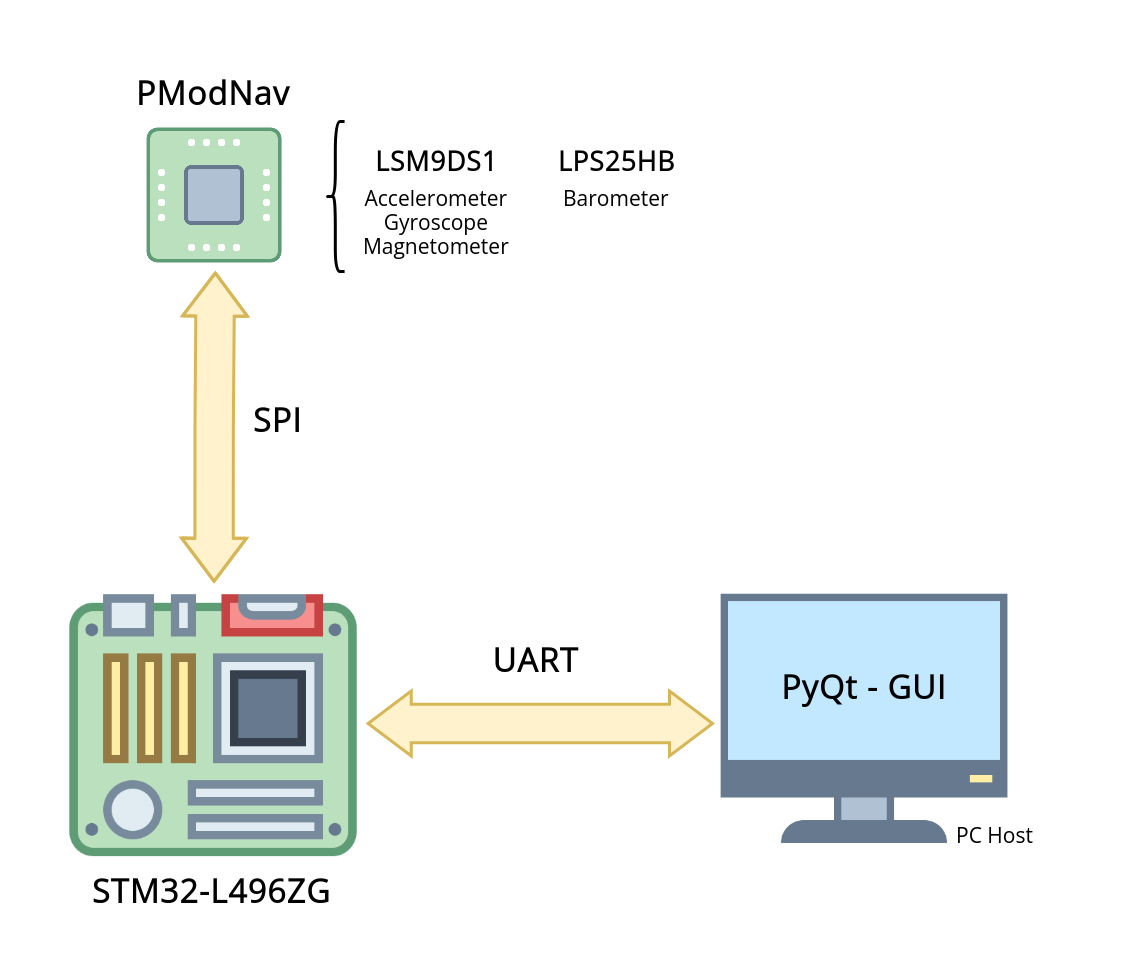
\includegraphics[width=0.65\linewidth]{./projects/pmodnav/com.png}
\end{center}

\subsubsection{Hardware}
The PModNav module is equipped with the LSM9DS1 sensor, offering 10-degrees-of-freedom (10-DOF) functionality. It integrates a 3-axis accelerometer, 3-axis gyroscope, 3-axis magnetometer, and an LPS25HB digital barometer. This comprehensive sensor suite allows users to obtain orientation-related data and determine the precise position and heading of the module. The module supports various full-scale options for linear acceleration, angular rate, and magnetic field measurements. It follows the Digilent Interface Specification Type 2A and utilizes a 12-pin Pmod connector with an SPI interface.

\subsubsection{Software and Development Environment}
The development environment for the PModNav project is STM32 CubeIDE. The documentation references project sources, including code snippets and libraries, such as the PModNav driver and Madgwick's filter implementation. 

\subsubsection{Data Processing}
The project outlines two approaches for deriving object attitudes: Euler angles and quaternions. Euler angles are obtained through the integration of angular velocity and provide information about the roll, pitch, and yaw of an object. However, a challenge known as "Gimbal Lock" arises when using Euler angles directly, resulting in a loss of a degree of freedom when two axes of rotation overlap. To overcome this, quaternions are introduced as a mathematical representation of displacement and rotation. They effectively resolve the Gimbal Lock issue and provide a more robust solution for determining attitudes.
\begin{center}
    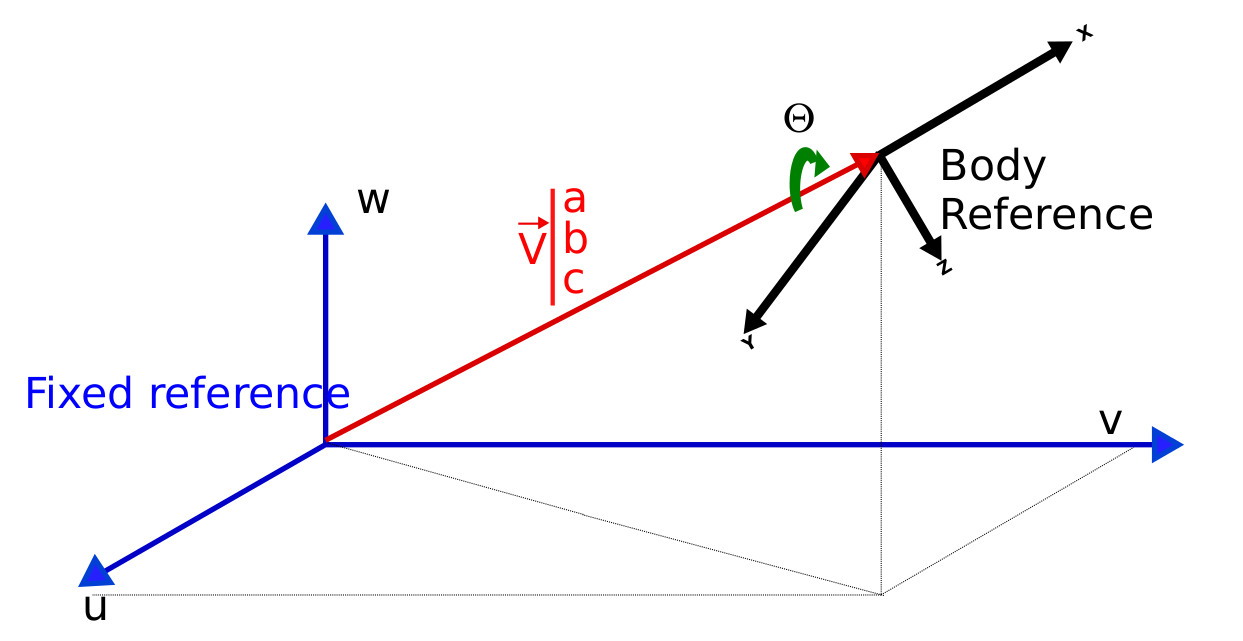
\includegraphics[width=0.65\linewidth]{./projects/pmodnav/quaternions.png}
\end{center}
$$ Q = [q_0, q_1, q_2, q_3 ] $$
$$ Q = \big[cos(\frac{\theta}{2}), a.sin(\frac{\theta}{2}), b.sin(\frac{\theta}{2}), c.sin(\frac{\theta}{2})\big] $$
At each \texttt{Te}, we can calculate the new value of the quaternion vector from the velocity :
$$ Q_{k+1} = Q_k+\frac{1}{2}.T_e.\omega_k.Q_k $$
For cheap IMUs, it is unavoidable to perform a data fusion to make the accelerometer compensate for the gyroscope defect. If using a Kalmann filter is possible, there are other (faster) algorithms like Madgwick's. The idea is to compensate for the gyroscope measurement error by modulating its values by the result of a comparison between an estimate of the gravity field and the measured gravity field (with the accelerometer).
\begin{center}
    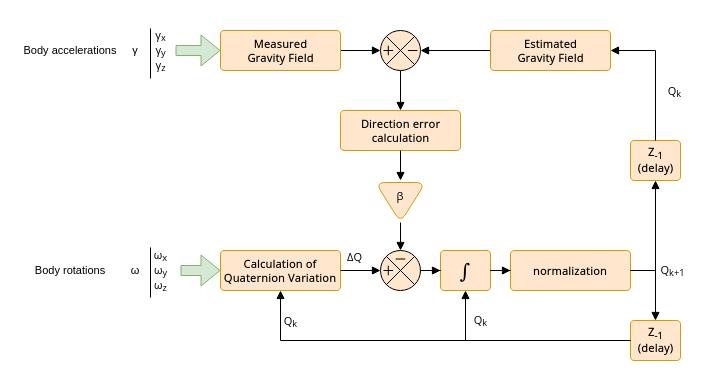
\includegraphics[width=0.9\linewidth]{./projects/pmodnav/madgwick.png}
\end{center}
I decided to use the most popular open source algorithm to compute rotations, the \texttt{Madgwick's algorithm}. This calculation updates the quaternion, from which the attitudes (Euler angles) can be calculated.
\begin{center}
    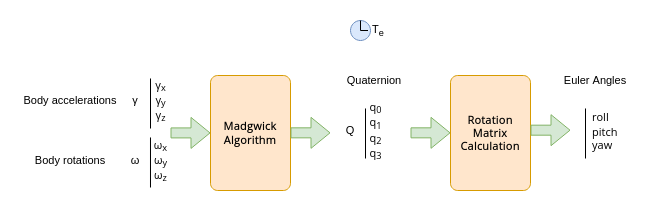
\includegraphics[width=0.9\linewidth]{./projects/pmodnav/madgwick_applied.png}
\end{center}
$$ R_{12} = 2.(q_1.q_2+q_0.q_3) $$
$$ R_{22} = q_0^2+q_1^2-q_2^2-q_3^2 $$
$$ R_{31} = 2.(q_0.q_1+q_2.q_3) $$
$$ R_{32} = 2.(q_1.q_3-q_0.q_2) $$
$$ R_{33} = q_0^2-q_1^2-q_2^2+q_3^2 $$
Calculation of the Euler Angles from the rotation matrix :
$$ roll = atan2(R_{12},R_{22}) $$
$$ pitch = atan2(R_{31},R_{33}) $$
$$ yaw = asin(R_{32}) $$


\subsection{Graphical User Interface}
Additionally, a graphical user interface (GUI) is provided, leveraging PyQt5 and PyOpenGL modules. The GUI manages the main window and handles OpenGL object management. It offers features like port selection and serial communication. The received data is displayed in a textbox within the GUI, facilitating real-time monitoring and analysis.
Here is how the GUI is threaded :
\begin{center}
    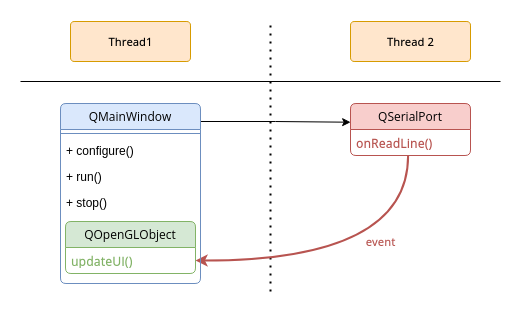
\includegraphics[width=0.65\linewidth]{./projects/pmodnav/gui_threads.png}
\end{center}
The use is rather simple for the communication configuration (\colorbox{cyan}{cyan box}) :
\begin{itemize}
    \item the port
    \item the baud rate
    \item the number of bits per frame
    \item the number of stop bits
    \item the parity
    \item the flow control
\end{itemize}
\begin{center}
    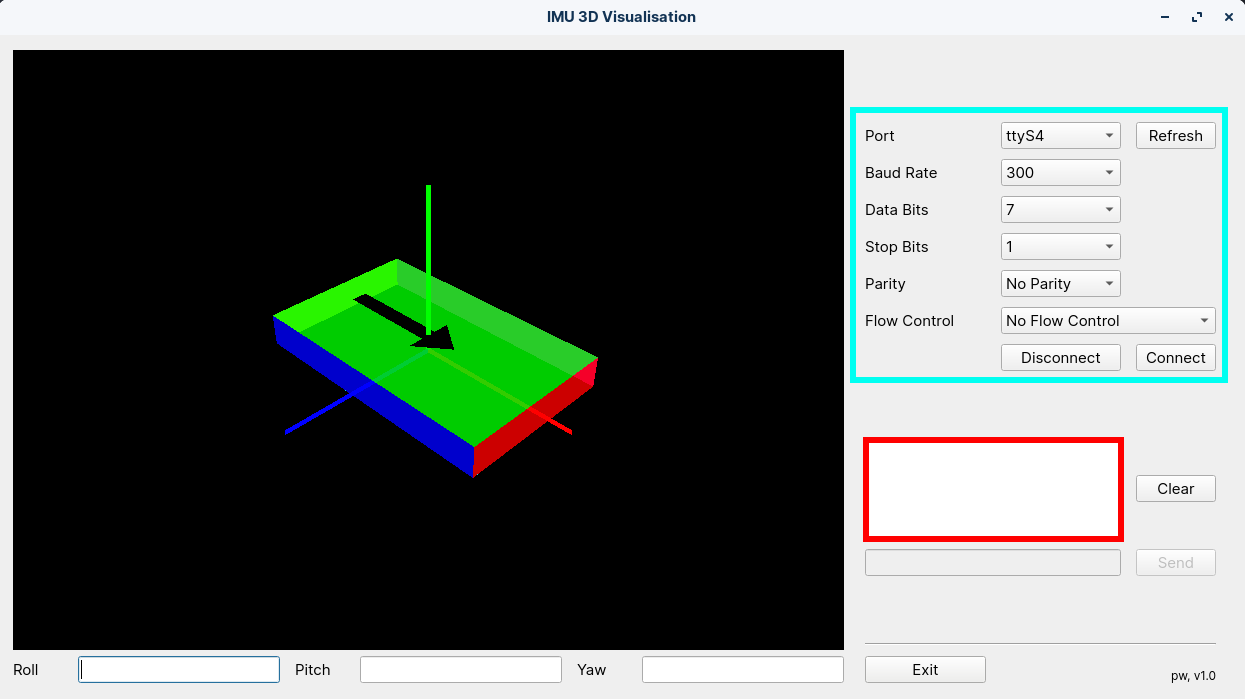
\includegraphics[width=0.65\linewidth]{./projects/pmodnav/gui_window.png}
\end{center}
Then click on \texttt{Connect} to start the serial communication. Every received line appeared in the textBox (\colorbox{red}{red box}).

\subsection{Final result}
% \begin{center}
%     \animategraphics[width=0.65\linewidth,autoplay,loop]{12}{projects/pmodnav/pmodnav_gui_record/pmodnav_gui_record-}{0}{299}
% \end{center}

\section{LogViewer}

\section{Collision avoidance SITL}

